\documentclass{article}

\usepackage[T1]{fontenc}
\usepackage{amsmath}
\usepackage{amssymb}
\usepackage{graphicx}
\usepackage{titling}
\usepackage{ragged2e}
\usepackage{lipsum}
\usepackage{booktabs}
\usepackage{fancyvrb}
\usepackage[hidelinks]{hyperref}
\usepackage[a4paper,left=0.75in,right=0.75in,top=1in,bottom=1in,footskip=0.5in]{geometry}

\pretitle{\vspace{1in}\hrulefill\par}
\posttitle{\par\hrulefill}

\title{\begin{center}\Huge COMP2432\\
    G06 Group Project Reoprt\end{center}}
\date{}
\author{}

\begin{document}
    \begin{titlepage}
        \maketitle
        \begin{center}
            \huge Room Booking Manager
            \vfill
            \begin{table}[!htbp]
                \centering
                \huge
                \begin{tabular}{ll}
                    19081789D\hspace{0.25in}&MAN, Furui \\
                    19078543D\hspace{0.25in}&WANG, Meng \\
                    18080998D\hspace{0.25in}&WU, Junyu  \\
                    19079008D\hspace{0.25in}&XING, Shiji\\
                \end{tabular}
            \end{table}
            \vspace{0.5in}
            \thispagestyle{empty}
        \end{center}
    \end{titlepage}
    \cleardoublepage
    \tableofcontents
    \thispagestyle{empty}
    \cleardoublepage
    \setcounter{page}{1}
    \section{Introdoction}
        \paragraph{}
        The project aims to utilize the knowledge covered in COMP2432 Operating Systems
        and put them into practice to get a further understanding and improvement. 
        This work is based on the scenario of implementing of a room booking manager
        for a frictional company, PolySME Bussiness center. By making advantage of
        various abstracted skills covered in the lecture , i.e. scheduling algorithms,
        multi-process programming, and interprocess communication a simple scheduler
        core and related utilities is developed.
    \cleardoublepage
    \section{Scope}
        \subsection{Multi-Process Programming and Inter-process Communication}
            \paragraph{}
            Scheduling module is implemented as a child process created via fork(). The communication between parent and scheduling module is based on pipe(), write(), and read(). In addition, in order to deliver complex information, we use pointers and pipes together. To utilize CPU, child processes are created for different scheduling methods, so that they can run at same time. The parent process uses read() and write() to synchronize among childern and to control the order of output. Additionally, since opti works on the basis of prio scheduling, the result of prio scheduling is directly passed to opti via mother process in order to avoid redundant computations.
        \subsection{ CPU Scheduling}
            \paragraph{}
            In this project, we are required to implement FCFS and prio algorithm for component booking, which is similar to what we learned in lectures about CPU Scheduling. However, there are some difference between algorithms in CPU scheduling and booking scheduling. In booking scheduling, we only care about the order of coming request and don't mind exact arrival time. In CPU scheduling, processes can be finished while in booking scheduling, requests can't be finished during the scheduling. Thus, the method to implement booking scheduling algorithms is similar to but still differs from CPU scheduling.
        \subsection{Memory Allocation}
            \paragraph{}
            Thinking of rooms as fixed partitions and requests as jobs, the process of allocating rooms for requests has the same logic as Multi-programming with a Fixed number of Tasks, where we have fixed amount of resources which is divided into certain numbers of partitions, and our task is to allocate different amounts of resources for objects in need of resources.
        \subsection{Synchronization}
            \paragraph{}
            Program-Monitored Synchronization is used for development. Since three children are running scheduling algorithms independently, some measure must be taken to synchronize and control the output. The parent process uses pipes to send signals to childs to control their behaviors, so that they can perform the scheduling algorithms simultaneously and be able to print results in order.
    \cleardoublepage
    \section{Concept}
        \subsection{FCFS Scheduling}
            \paragraph{}
                First-Come-First-Serve(aka, FCFS) handles requests upon a first-come-first-serve basis. Later requests that cause collision are rejected, otherwise are accepted.
            \paragraph{}
                In its implementation, no sorting is needed because the order of the request link-list during scheduling is exactly the same as that of input, given that the invalid ones have been filtered out. The only thing to note is that to maintain the order of requests, Input-Handler Module must be single-threaded.
            \paragraph{}
                Below is a illustration of FCFS algorithm. Green-colored requests are accepted, whereas red-colored requests are rejected, and the requests arrive in sequence indicated by arrows between. 
            \begin{figure}[!htbp]
                \centering
                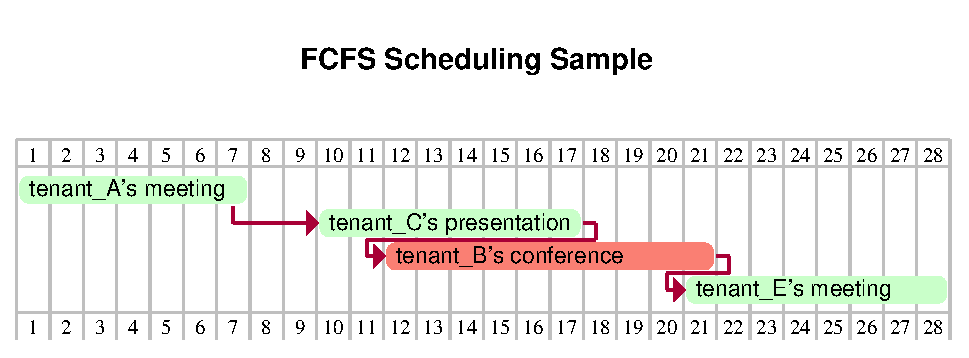
\includegraphics[scale=0.7]{../res/eps/fcfs_scheduling.eps}
                \caption{Gantt Diagram for FCFS algorithm Sample output for one single Room}
            \end{figure}
        \subsection{PRIO Scheduling}
            \paragraph{}
            Priority scheduling(aka, PRIO) is the scheduling algorithm based on the
                priority of requests. Rather than that in FCFS which indicated by arriving time, the priority are implied within the requests weighted by its type (i.e. device-booking, meeting, presentation, or conference). 
            \paragraph{}
            To implement PRIO, the tasks required is to stably sort the request link-list upon user-defined priority, then call FCFS scheduling. This would reuse the code and decrease the overall complexity of the program.
                Requests are stored in an array after sortion based on priority. 
            \paragraph{}
            Below is the visualization of PRIO scheduling, with the same annotation rules as used in FCFS.
            \begin{figure}[!htbp]
                \centering
                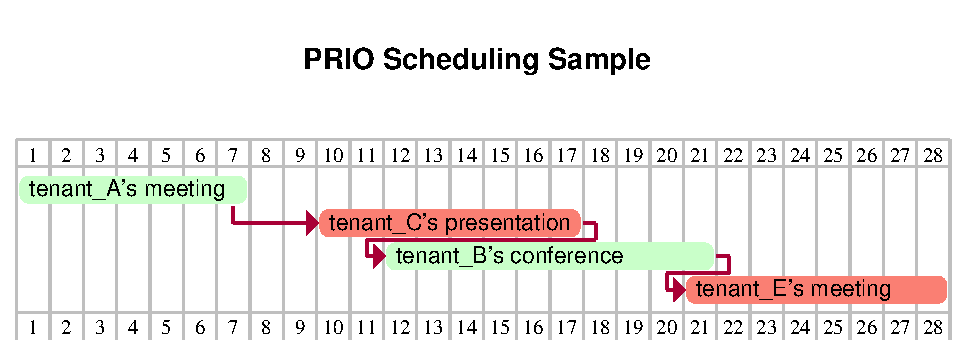
\includegraphics[scale=0.7]{../res/eps/prio_scheduling.eps}
                \caption{Gantt Diagram for PRIO algorithm Sample output for one single Room}
            \end{figure}
        \subsection{OPTI Scheduling}
            \paragraph{}
                Optimized Scheduling bases on the result of PRIO or FCFS scheduling and it rescheduled the valid failed requests. The process first finds a desired time slot  of a rejected request, and try to "push" this time slot to both sides until it finds a suitable time slot for this request. Then it selects one that is closer to the original desired time slot and update the request. The process repeats this procedure untill all requests that can be rescheduled is rearranged.
    \cleardoublepage
    \section{Algorithm}
    \subsection{Design of own algorithm}
        \paragraph{Optimization Algorithm}
        \paragraph{}
            Optimization algorithm is based on processed result by FCFS algorithm or
            PRIO algorithm. Failed requests from the two algorithm firstly undergo
            verification. Valid requests are rescheduled based on bi-directional
            search of linked lists of rooms and devices. 

    \cleardoublepage

    \section{Program Structure}
        \subsection{Class Design}
            \begin{figure}[!htbp]
                \centering
                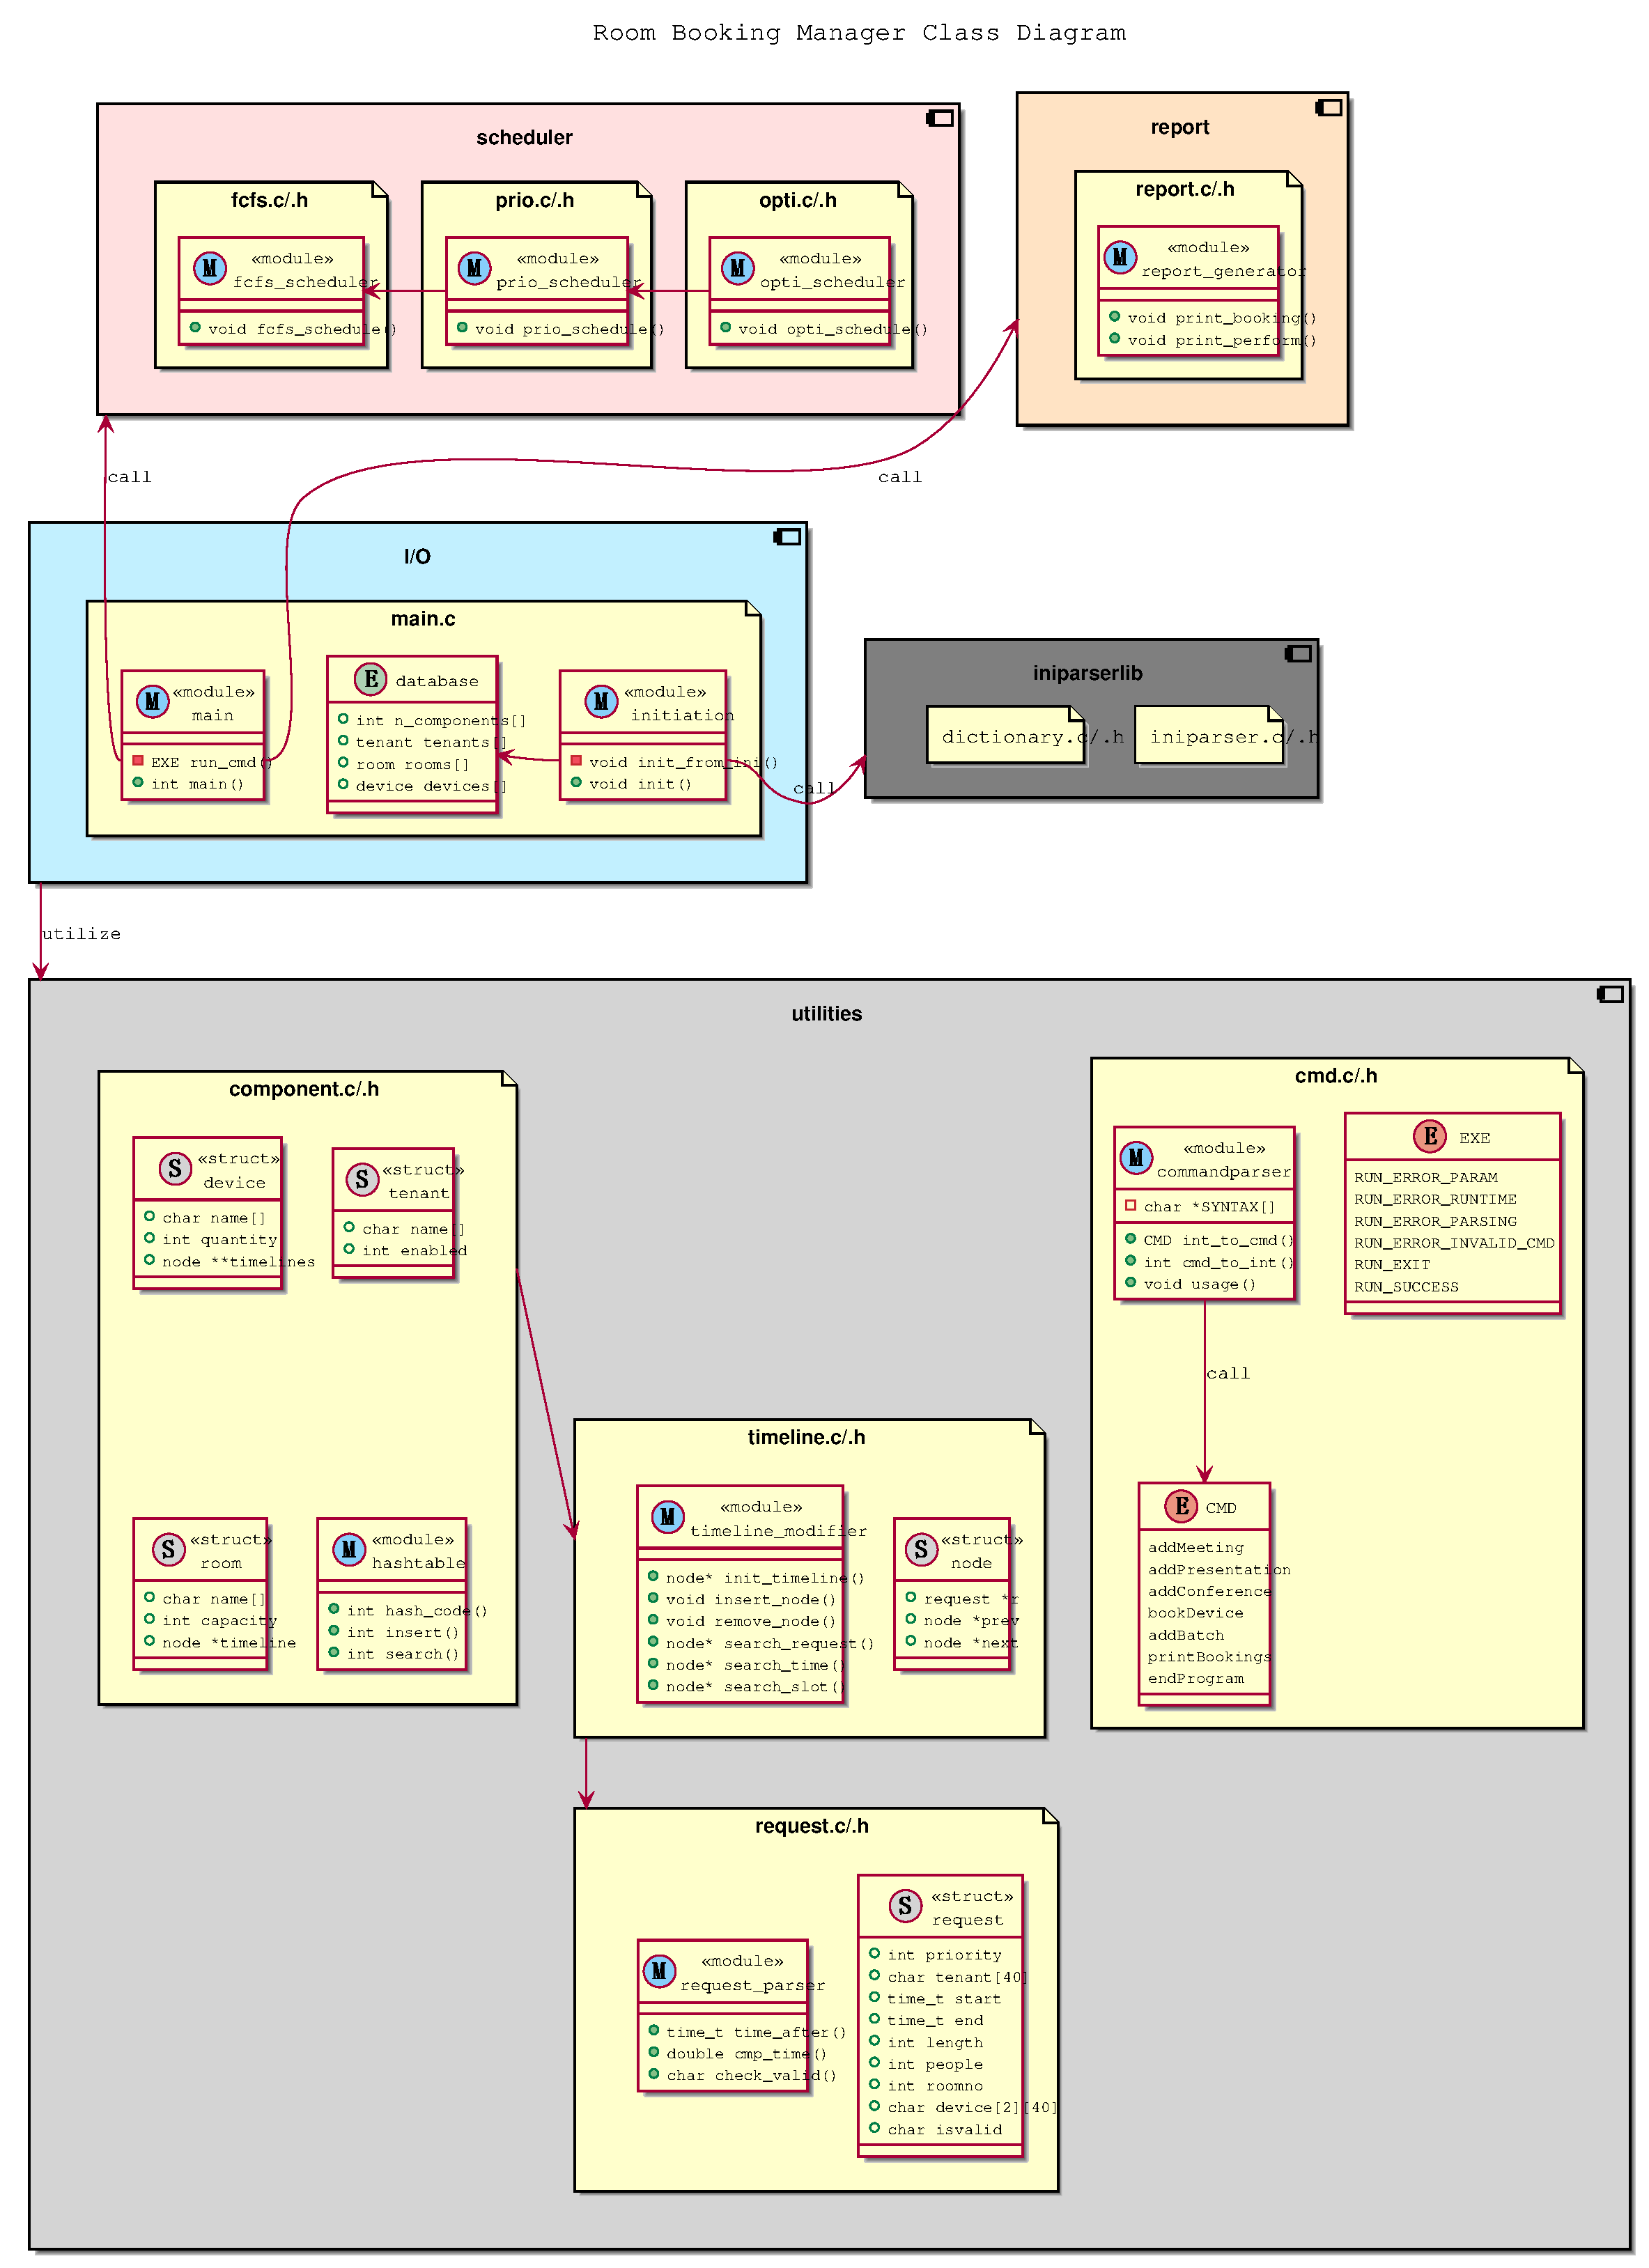
\includegraphics[scale=0.4]{../res/eps/class_diagram.eps}
                \caption{Overall class design diagram of Room Booking Manager}
            \end{figure}
        \subsection{Sequence Design}
            \begin{figure}[!htbp]
                \centering
                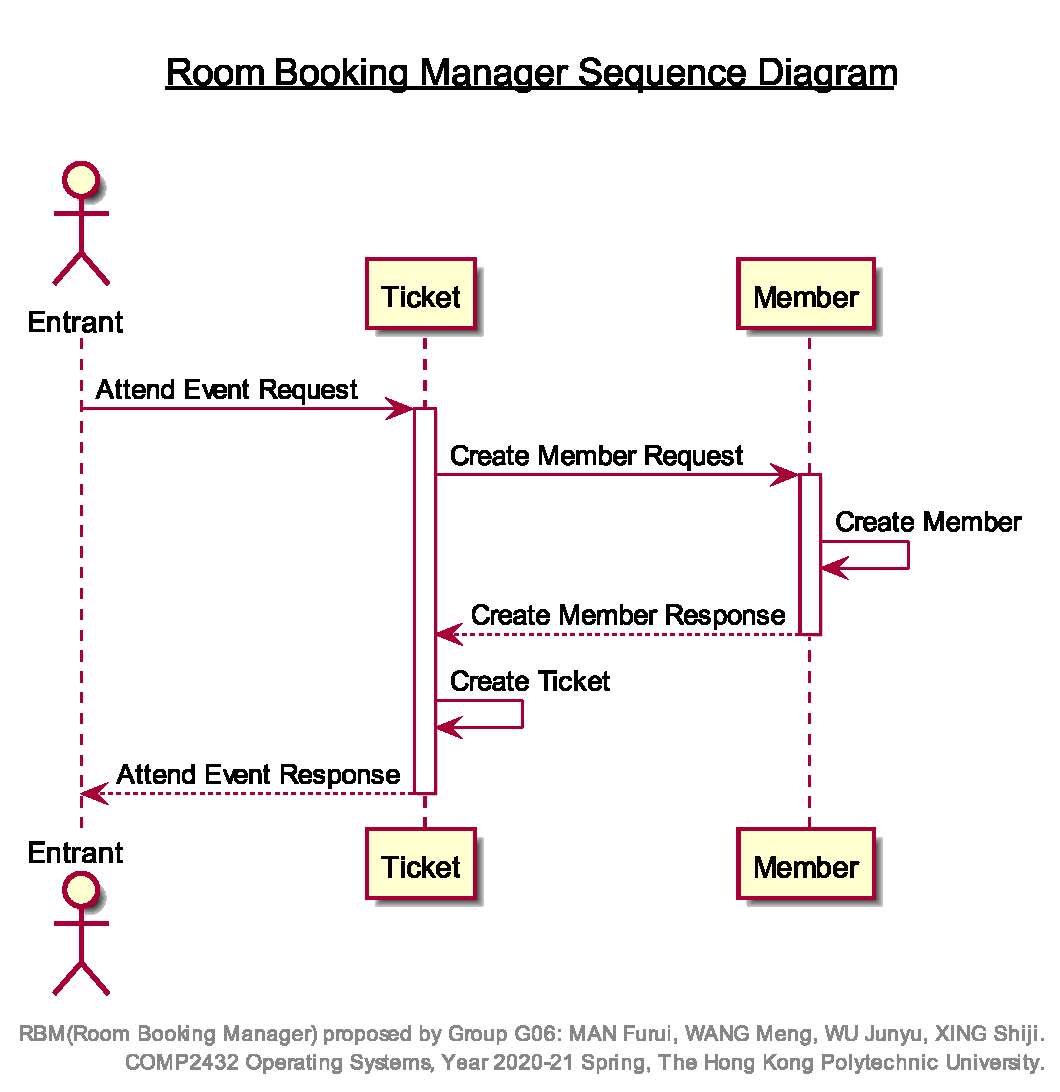
\includegraphics[scale=0.5]{../res/eps/sequence_diagram.eps}
                \caption{Overall sequence design diagram of Room Booking Manager}
            \end{figure}
        \subsection{Activity Design}
            \begin{figure}[!htbp]
                \centering
                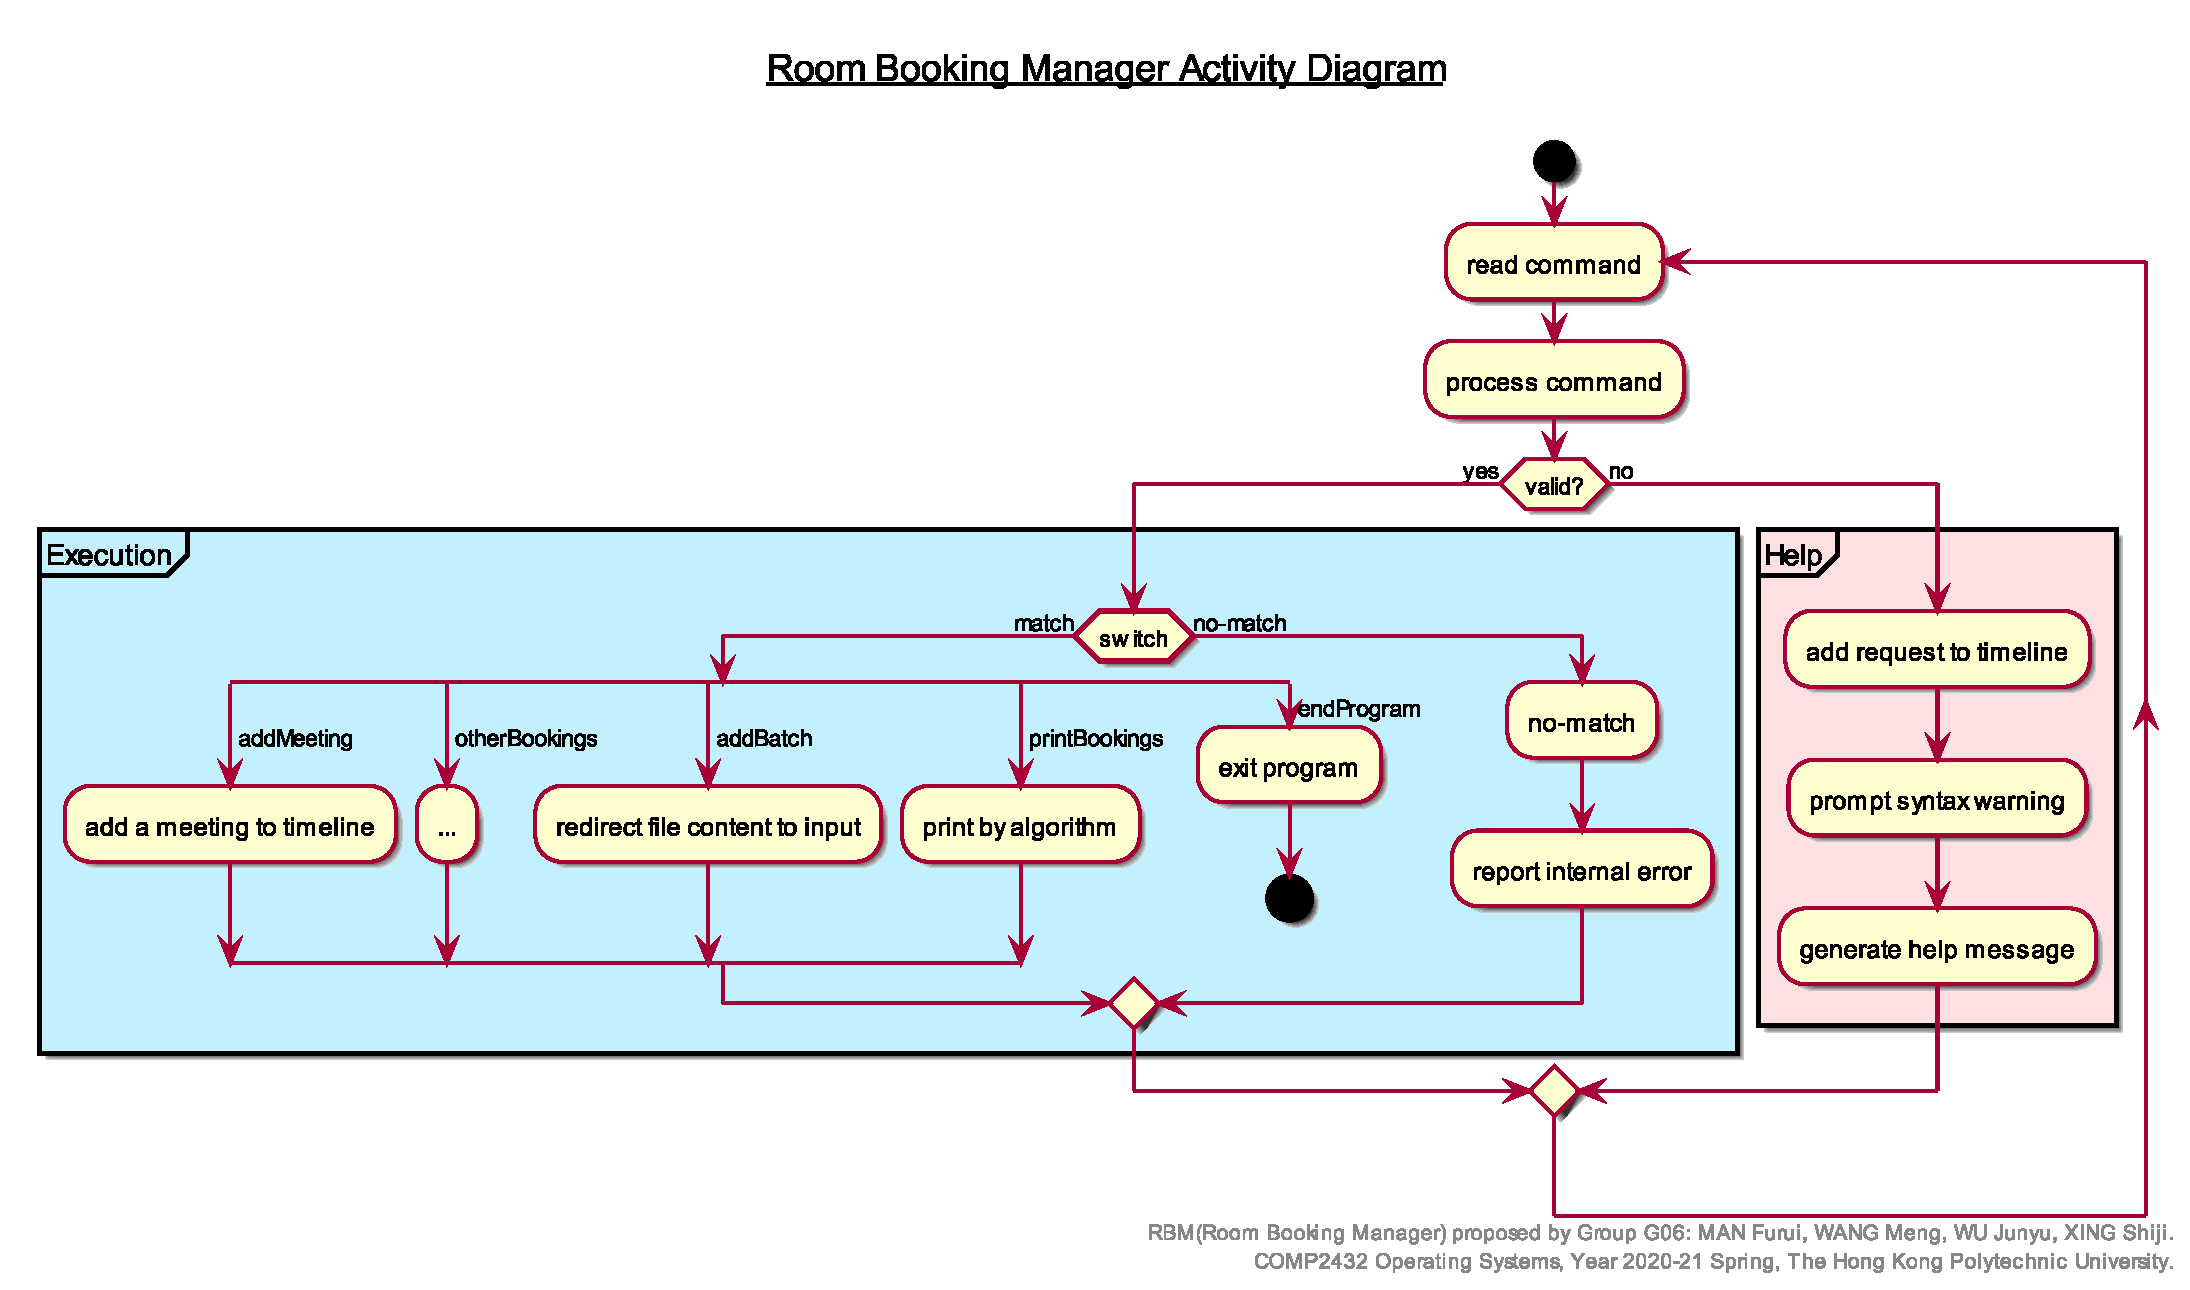
\includegraphics[scale=0.45]{../res/eps/activity_diagram.eps}
                \caption{Overall activity design diagram of Room Booking Manager}
            \end{figure}
    \cleardoublepage
    \section{Testing Cases}
        \paragraph{}
        This is the brief version, which demonstrates the valid and invalid tests for \texttt{addMeeting} instruction only.
        \paragraph{}
        Tests for other instructions are similar and therefore not included. Syntax of other instructions varies in
        number of the parameters. Help message on syntax is available once an input error is detected.
        \paragraph{}
        Refer to the appendix for the full version. 

        \subsection{Valid Tests}
            \paragraph{}
            Valid syntax for \texttt{addMeeting} instruction should be:
            \begin{Verbatim}[gobble=8]
                addMeeting -tenant YYYY-MM-DD hh:mm n.n [d1 d2]; 
            \end{Verbatim}
            \paragraph{}
            Below are some samples which conforms the above syntax:
            \begin{Verbatim}[gobble=8]
                addMeeting -tenant_A 2021-05-10 21:50 1.50 5 projector_2K screen_100;
                addMeeting -tenant_A 2021-05-11 18:20 0.30 5;
                addMeeting -tenant_A 2021-05-11 4:10 0.0 5;
            \end{Verbatim}
        
        
        \subsection{Invalid Tests}
            \paragraph{}
            Invalid instructions of addMeeting contains either:
            
            \begin{itemize}
            \item Syntax invalid: (including command invalid, tenant invalid, date invalid, hour and minute invalid,
            duration invalid, number of people invalid, device invalid); or
            \end{itemize}
            
            \begin{Verbatim}[gobble=8]
                command_invalid and parameters does not matter;
                addMeeting -tenant_invalid 2021-05-10 1:30 0.50 5 projector_2K screen_100;
                addMeeting -tenant_A date-in-valid 1:30 0.50 5 projector_2K screen_100;
                addMeeting -tenant_B 2021-05-10 hhmm:invalid 1.50 5 webcam_FHD monitor_75;
                addMeeting -tenant_C 2021-05-10 18:30 duration.invalid 5 webcam_FHD monitor_50;
                addMeeting -tenant_D 2021-05-10 10:40 0.0 peopleinvalid projector_2K screen_150;
                addMeeting -tenant_D 2021-05-16 3:10 1.10 5 device_invalid monitor_50;
            \end{Verbatim}
            \begin{itemize}
            \item Device pairing error (devices must be in pairs).
            \end{itemize}
            \begin{Verbatim}[gobble=8]
                addMeeting -tenant_E 2021-05-10 22:20 0.50 5 projector_4K monitor_50; 
                addMeeting -tenant_E 2021-05-10 22:20 0.50 5 projector_4K; 
            \end{Verbatim}
        

    \cleardoublepage
    \section{Performance analysis}

    \cleardoublepage
    \section{Program Setup \& Analysis}
        \subsection{Program Setup}
            \paragraph{Step 0 Clone repo (optional)}
            \paragraph{}
                Clone the repo from Github if there is no local copy.
            \begin{Verbatim}[gobble=8]
                git clone https://github.com/toolsmax0/COMP2432_RBM.git
            \end{Verbatim}
            \paragraph{Step 1 Compilation}
            \paragraph{}
                \texttt{cd} to the project's root directory and execute \texttt{build.sh} script.
            \paragraph{}
                The program have dependency upon \texttt{gcc 4.0+} and \texttt{linux 3.0+}.
            \begin{Verbatim}[gobble=8]
                cd COMP2432_RBM
                sh build.sh
            \end{Verbatim}
            \paragraph{Step 2 Customization (optional)}
            \paragraph{}
                To modify the component settings (i.e. tenants, rooms, devices),
                modify \texttt{RBM.ini} file according to its syntax.
            \paragraph{Step 3 Execution}
            \paragraph{}
                To execute the program, run the following command.
            \begin{Verbatim}[gobble=8]
                ./out/RBM
            \end{Verbatim}

        \subsection{Progarm Analysis}
            
    \cleardoublepage
    \section{Appendix}
        \subsection{Source Code}
            \paragraph{}
                All source files are located under \texttt{./src/} directory. Please \texttt{cd}
                to corresponding directory for reference.
            \begin{Verbatim}[gobble=8]
                Insert source here
            \end{Verbatim}
        \subsection{Test Data}
            \paragraph{}
                All test data are generated with \texttt{generator.py} under \texttt{./test/}
                directory. Sufficient amount of test cases are generated via this generator
                and stored into \texttt{*.dat} files.
            \paragraph{}
                All files of test data are located under \texttt{./test/} directory. Please
                \texttt{cd} to corresponding directory for reference.
            \paragraph{}
                Files marked with \texttt{*\_invalid.dat} are invalid tests for specific command
                types. The rest of files are for valid tests.
            \begin{Verbatim}[gobble=8]
                Insert test data here
            \end{Verbatim}
        \subsection{Test Results}
            \paragraph{}
                Warnings should be generated for each invalid case, while not for valid cases. 
            \paragraph{}
                The descriptions of valid/invalid tests have been clearly stated under
                \textbf{9.2 Test Data}.
            \begin{Verbatim}[gobble=8]
                Insert warning here
            \end{Verbatim}
        \subsection{Sample Output}
            \paragraph{}
                Output of test files are stored in \texttt{sample\_output\_*.txt} file under
                \texttt{./test/} directory with algorithm applied. Please refer to the
                corresponding file for reference.
            \begin{Verbatim}[gobble=8]
                Insert Output file here
            \end{Verbatim}
\end{document}